\documentclass[a4paper,12pt]{article}
\usepackage[utf8]{inputenc}
\usepackage[italian]{babel}
\usepackage{amsfonts}
\usepackage{listings}
\usepackage{xcolor}
\usepackage{booktabs}
\usepackage{graphicx}
\usepackage{float}
\setcounter{tocdepth}{4}
\setcounter{secnumdepth}{4}

\title{Maps}
\author{Appunti di Programmazione}
\date{\today}

\begin{document}
\tableofcontents
\newpage

\maketitle

\section{AVL Trees}

\begin{figure}[H]
    \centering
    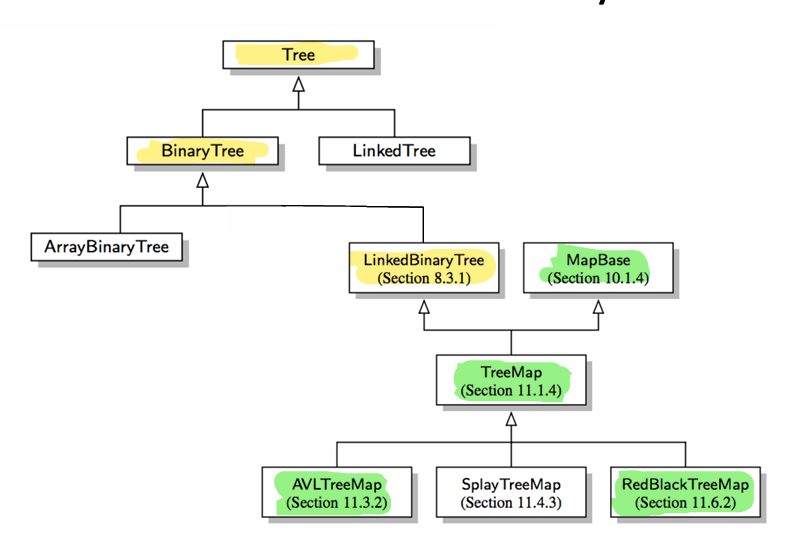
\includegraphics[width=0.7\linewidth]{Immagini/avlrbHierarchy.png}
    \caption{Gneral hierarchy}
\end{figure}

\newpage
\subsection{Balanced Tree}
Si suppone che il nodo foglia abbia altezza pari a 1.
\begin{figure}[H]
    \centering
    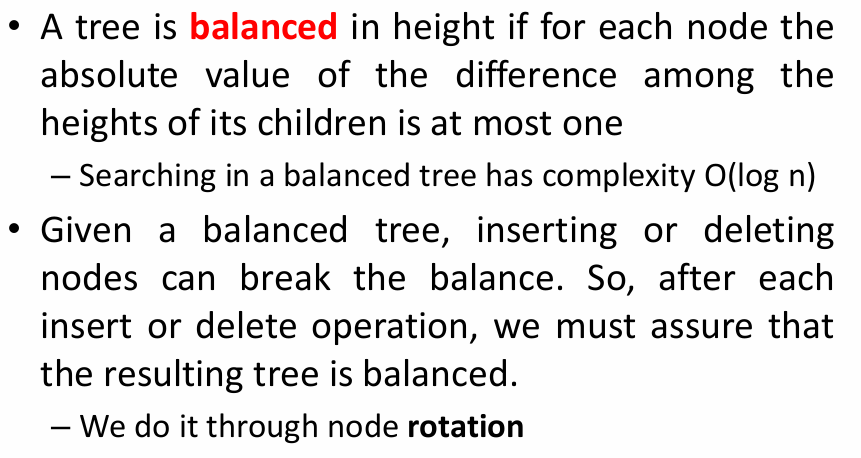
\includegraphics[width=0.47\linewidth]{Immagini/BalancedTree.png}
    \vline
    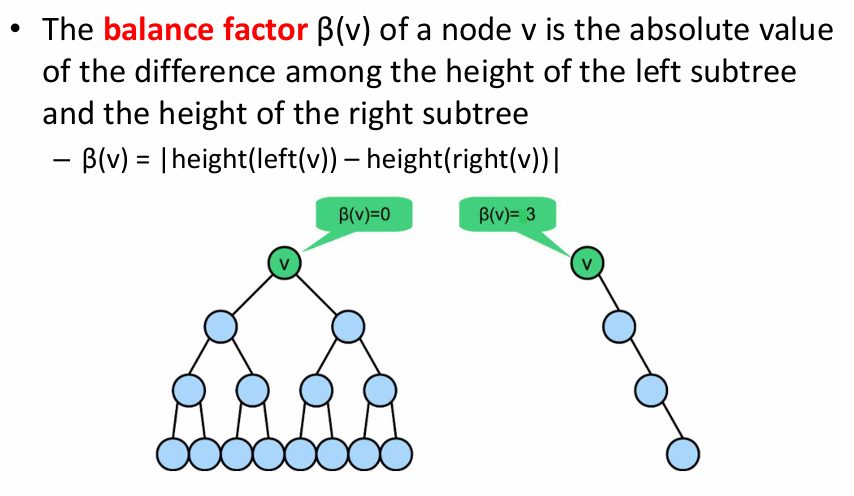
\includegraphics[width=0.47\linewidth]{Immagini/BalanceFactor.png}
    \caption{Balanced Tree Definition}
\end{figure}

\newpage
\subsection{AVL Tree definition}

\begin{figure}[H]
    \centering
    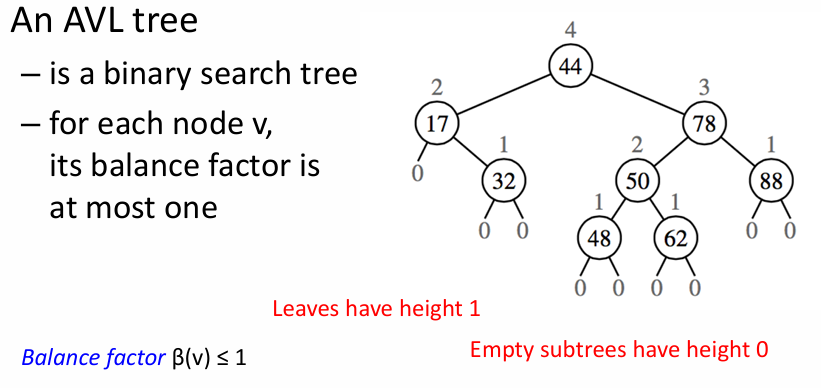
\includegraphics[width=0.47\linewidth]{Immagini/AVLDefinition.png}
    \vline
    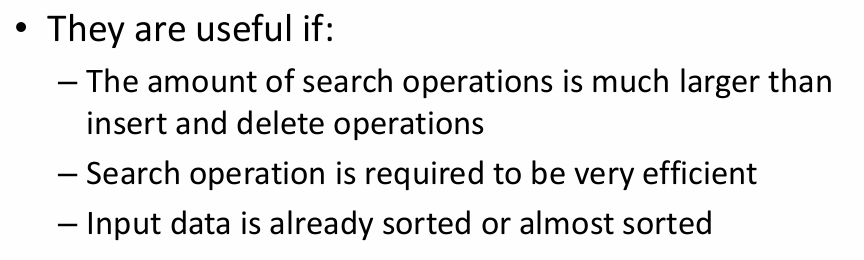
\includegraphics[width=0.47\linewidth]{Immagini/UsefulnessAVLtree.png}
    \caption{AVL Tree Definition}
\end{figure}

\newpage
\subsection{AVL Tree Rotations}
Per garantire che l'AVL tree rimanga bilanciato dopo inserimenti e cancellazioni, c'è bisogno di \textit{ruotare} i nodi.

\begin{figure}[H]
    \centering
    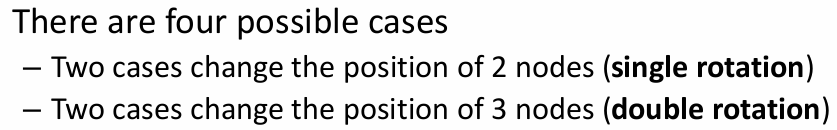
\includegraphics[width=0.7\linewidth]{Immagini/RotationCasesAVL.png}
    \caption{AVL Tree Rotations Cases}
\end{figure}

\subsubsection{First \& Second Case}
\begin{figure}[H]
    \centering
    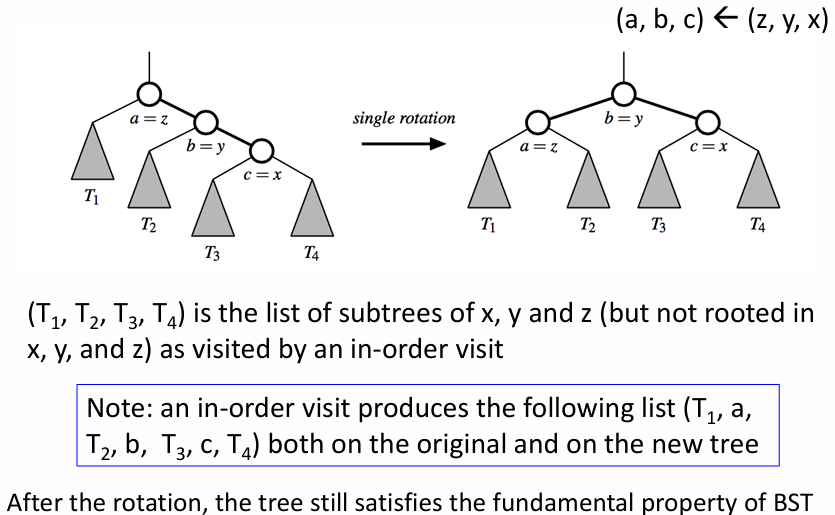
\includegraphics[width=0.47\linewidth]{Immagini/FirstCaseAVL.png}
    \vline
    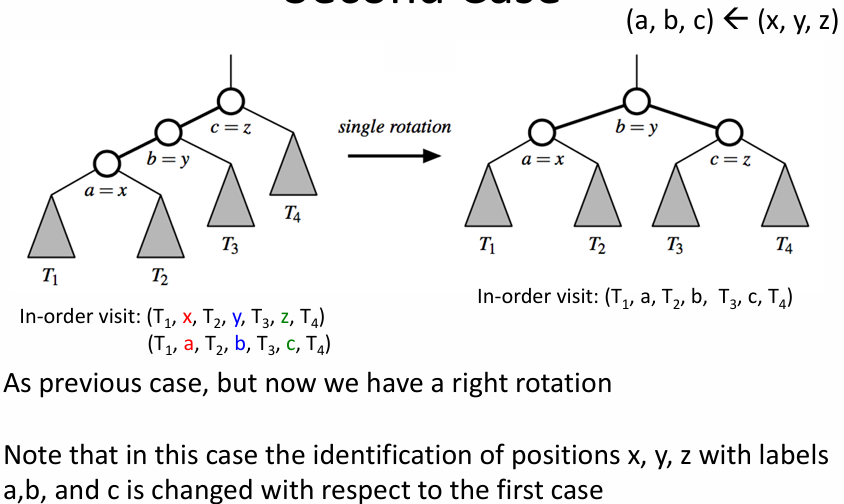
\includegraphics[width=0.47\linewidth]{Immagini/SecondCaseAVL.png}
    \caption{First \& Second Case}
\end{figure}

\subsubsection{Third \& Fourth Case}
\begin{figure}[H]
    \centering
    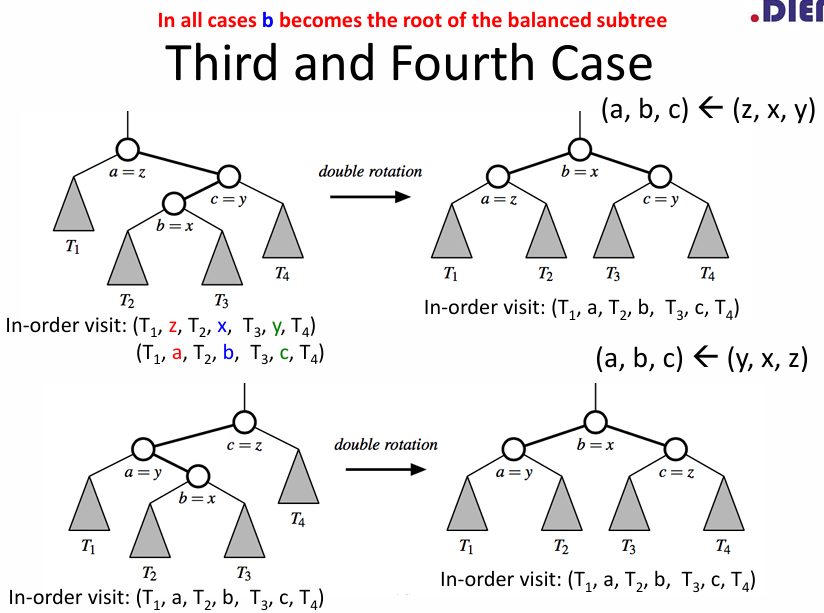
\includegraphics[width=0.47\linewidth]{Immagini/ThirdFourtCaseAVL.png}
    \vline
    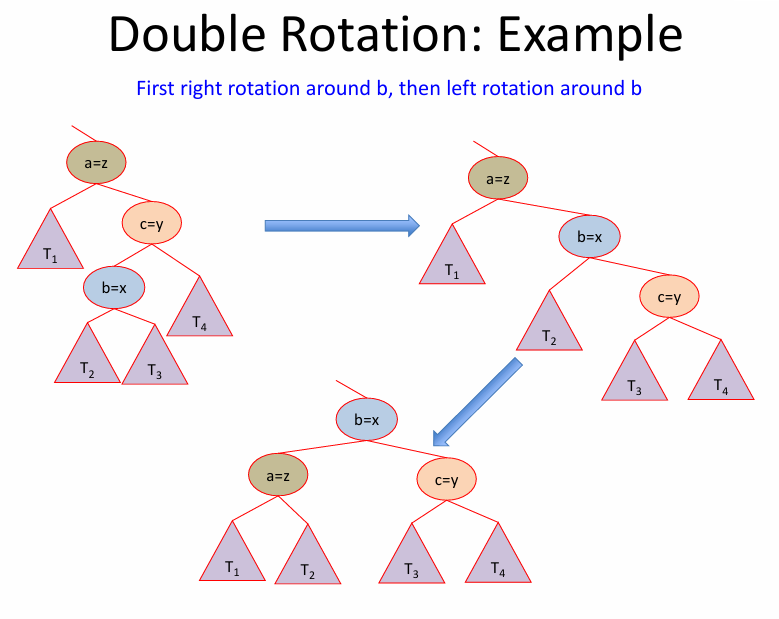
\includegraphics[width=0.47\linewidth]{Immagini/DoubleRotationAVL.png}
    \caption{Third \& Fourth Case}
\end{figure}

\subsection{Performance}

\begin{figure}[H]
    \centering
    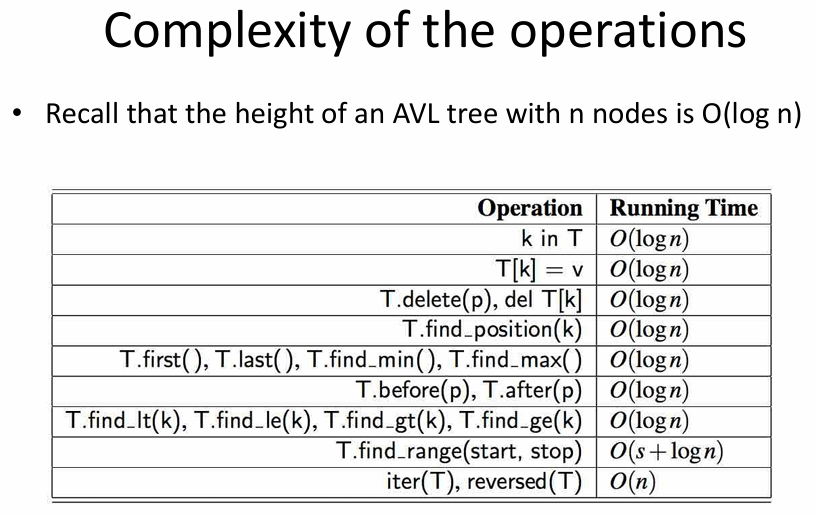
\includegraphics[width=0.47\linewidth]{Immagini/AVLPerformance.png}
    \vline
    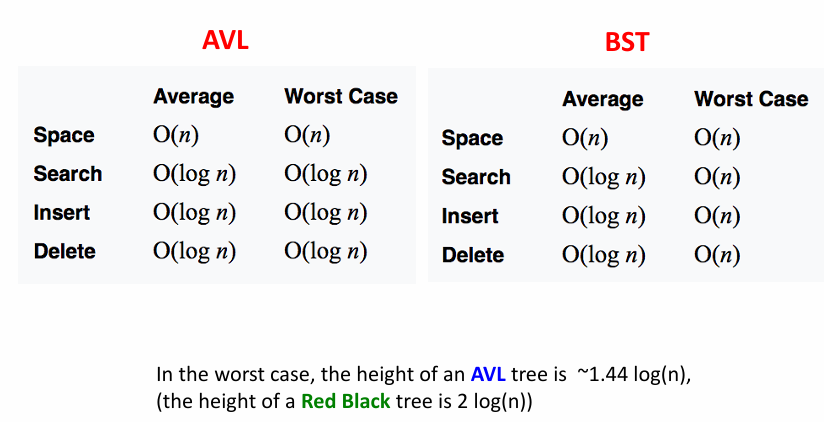
\includegraphics[width=0.47\linewidth]{Immagini/AVLPerformance2.png}
    \caption{AVL Tree Performance}
\end{figure}




\end{document}